\documentclass[
]{article}

\usepackage[utf8]{inputenc}

\providecommand{\tightlist}{%
  \setlength{\itemsep}{0pt}\setlength{\parskip}{0pt}}

\author{
Michiel Stock\\Ghent University \And Joris Meys\\Ghent University \And Bernard De Baets\\Ghent University
}
\title{Predicting Networks With Two-Step Kernel Ridge Regression: The R Package
\pkg{xnet}}

\Plainauthor{Michiel Stock, Joris Meys, Bernard De Baets}
\Plaintitle{Predicting Networks With Two-Step Kernel Ridge Regression: The R Package
\texttt{xnet}}
\Shorttitle{\pkg{xnet}: Cross-validating Two-Step Kernel Ridge Regression}

\Abstract{
This paper presents the R package \pkg{xnet} for cross-network analysis
of bipartite networks, using two-step kernel ridge regression. It uses
the cross-validation shortcuts proposed by \citet{stock2018} to allow
for computationally efficient evaluation of the models based on a
variety of leave-one-out methods. The package provides functions for
easy tuning, fitting, and evaluation of two-step kernel ridge regression
in the context of cross-network analysis. We illustrate the use of the
\pkg{xnet} package with datasets from different areas of research.
}

\Keywords{networks, pairwise learning, cross-validation, kernel methods}
\Plainkeywords{networks, pairwise learning, cross-validation, kernel methods}

%% publication information
%% \Volume{50}
%% \Issue{9}
%% \Month{June}
%% \Year{2012}
%% \Submitdate{}
%% \Acceptdate{2012-06-04}

\Address{
    Michiel Stock\\
  Ghent University\\
  KERMIT, Department of Data Analysis and Mathematical Modelling
  \newline Coupure Links 653 B-9000 Gent Belgium\\
  E-mail: \email{michiel.stock@ugent.be}\\
  URL: \url{https://www.ugent.be/bw/damm/en}\\~\\
      Joris Meys\\
  Ghent University\\
  Department of Data Analysis and Mathematical Modelling \newline Coupure
  Links 653 \newline B-9000 Gent, Belgium\\
  E-mail: \email{Joris.Meys@UGent.be}\\
  URL: \url{https://www.ugent.be/bw/damm/en}\\~\\
      Bernard De Baets\\
  Ghent University\\
  KERMIT, Department of Data Analysis and Mathematical Modelling
  \newline Coupure Links 653 B-9000 Gent Belgium\\
  E-mail: \email{bernard.debaets@ugent.be}\\
  URL: \url{https://www.ugent.be/bw/damm/en}\\~\\
  }

% Pandoc header

\usepackage{amsmath,amssymb} \usepackage{tikz}

\usetikzlibrary{shapes.geometric,arrows}

\usepackage{pgf,tikz,pgfplots}

\pgfplotsset{compat=1.15} \usetikzlibrary{matrix}

\begin{document}

\hypertarget{introduction}{%
\section{Introduction}\label{introduction}}

Networks or graphs\footnote{The term `network' is prevalent in sciences,
  whereas `graph' is a term predominantly used in mathematics and formal
  computer science. In this work, we will use both interchangeably.} are
one of the most powerful tools to represent complex, structured
information. It is no wonder that nearly all sciences ubiquitously use
networks; from chemistry (e.g., molecular graphs), to molecular biology
(e.g., protein-interaction networks), to ecology (e.g., plant-pollinator
networks), to sociology (e.g., social networks). On the one hand, graphs
can be seen as minimalistic mathematical models, conveying how
individual components in a system are connected. On the other hand,
graphs are also data structures; they can be constructed by performing
experiments or gathering observational data.

Given the general importance of graphs, a plethora of machine learning
methods has been developed to predict networks based on data. We can
divide network prediction methods into two groups: unsupervised and
supervised. Unsupervised network inference, also called \emph{de novo}
inference \citep{Vert2008}, do not use a dataset of known interactions
to predict the network. These methods are often based on the
guilt-by-association principle: components that occur together in space
or time are assumed to interact. Such approaches are commonly used in
computational biology, in particular for inferring gene regulatory
networks (e.g., \citet{Huynh-Thu2010}; \citet{Marbach2012};
\citet{Maetschke2014}) or to infer species interaction networks from
co-occurrence data (e.g., \citet{Basnou2015}; \citet{Cazelles2016}).
Recently, however, a study found that correlation-based methods perform
poorly to uncover the underlying network, at least for virus-bacteria
networks \citep{Coenen2018}. Furthermore, a significant limitation of
the unsupervised methods is that they are unable to generalize beyond
the original data: they are not capable of prediction interactions for
previously unobserved nodes.

Supervised network prediction methods depart from an initial network
that is used for training a machine learning model. This model then can
predict interactions for nodes within or outside the training network.
For even a small number of example interactions, supervised methods are
observed to outcompete their unsupervised counterparts
\citep{Cazelles2016}. Supervised network prediction methods are
particularly popular in molecular network prediction -- see
\citet{Vert2008} and \citet{Ding2013} for an overview. In this work, we
will often refer to supervised network prediction using the more general
term \emph{pairwise learning}: predicting properties of pairs of objects
using machine learning. \emph{In casu}, predicting the edge between two
nodes.

We present our R-package \textbf{xnet}, a simple, but flexible toolbox
for performing pairwise learning using two-step kernel ridge regression
\citep{Jung2013, Pahikkala2014a, Romera-paredes2015}. Two-step kernel
ridge regression is a straightforward combination of two standard kernel
ridge regression methods to extend these to pairwise learning. This
method yields a bilinear prediction model, capable of learning
arbitrarily complex relations between two objects. Such models have been
used excessively in molecular network prediction, e.g.,
\citet{Vert2007};\citet{VanLaarhoven2011a};\citet{Pahikkala2015};\citet{Pelossof2015}
as well as for more general problems
\citep{Brunner2012, Pahikkala2013a, Liu2015a}.

Due to its simplicity, the two-step kernel ridge regression method has
many computational advantages compared to other methods. It can be
fitted exceptionally efficiently for large datasets, and the
regularization parameters can be changed at no additional cost
\citep{Stock2017tskrr}. Furthermore, performing leave-one-out
cross-validation for the different prediction settings that arise in
pairwise learning can also be done at constant time complexity provided
that a model is pretrained \citep{Stock2017tskrr}. Finally, we provide
the functionality to assess variable importance, impute missing values,
and visualize the model. The connection with other packages for
computing kernel matrices ensures that \textbf{xnet} can cope with a
wide variety of complex and possibly structured data.

The remainder of this work is structured as follows. In Section
\ref{sec:snp}, we give a short, self-contained background to
kernel-based pairwise learning and two-step kernel ridge regression. The
API of the package is demonstrated in \ref{sec:useofpackage} while
Section \ref{sec:relatedsoftware} provides some pointers to related
software. Finally, some small case studies are presented in
\ref{sec:casestudy}.

\hypertarget{supervised-network-prediction}{%
\section{Supervised network
prediction}\label{supervised-network-prediction}}

\label{sec:snp}

In this section, we will give an overview of the methods provided by
\texttt{xnet}. First, we explain how two-step kernel ridge regression
for pairwise learning can be motivated from standard kernel ridge
regression. The next section discusses how two-step kernel ridge
regression can be used when the data is not complete, i.e., there is not
exactly one training pair for each possible combination. The final
section handles model selection and validation. We discuss
cross-validation schemes and permutation methods tailored to the
pairwise prediction setting to correctly assess the performance of the
models. This section is meant to be introductive. We refer to standard
works and original publications for in-depth motivations, derivations,
and discussion of the various methods.

\hypertarget{pairwise-learning-with-kernels}{%
\subsection{Pairwise learning with
kernels}\label{pairwise-learning-with-kernels}}

\hypertarget{kernel-ridge-regression}{%
\subsubsection{Kernel ridge regression}\label{kernel-ridge-regression}}

Classical supervised machine learning methods depart from a
\emph{labeled training set}. The training \(T\) set is a set of \(l\)
labeled instances
\(T = \{(x_k, y_k)\mid i=1,\ldots,l\} \in (\mathcal{X}\times \mathcal{Y})^l\).
Here, \(\mathcal{X}\) denotes the space of the \emph{instances} (also
called cases, observations or inputs) and \(\mathcal{Y}\) the
\emph{labels} (also called targets or outputs). In this work, we assume
that \(\mathcal{Y}\) is numeric, i.e., the label could be real-valued,
resulting in a \emph{regression problem} or binary, resulting in a
\emph{binary classification problem}.

The goal of supervised learning if to find a suitable \emph{prediction
function} \(f : \mathcal{X}\rightarrow\mathcal{Y}\) such that
\(f(x_k) \approx y_k\) for all \(k\). A vital step in designing
prediction function is choosing a suitable feature mapping
\(\phi:\mathcal{X}\rightarrow \mathcal{H}\) of the instances. This
function links the abstract space of the instances to a concrete Hilbert
space \(\mathcal{H}\) in which the supervised learning problem is easy
to solve. Depending on the data, \(\phi(\cdot)\) might be a nonlinear
function, and \(\mathcal{H}\) could be of very large or even infinite
dimension.

Rather than designing a feature map explicitly, \emph{kernel methods}
construct a Hilbert space by implication \citep{Scholkopf2002}. A
\emph{kernel function} is a symmetric and positive-definite function
\(\Gamma : \mathcal{X} \times \mathcal{X} \rightarrow \mathbb{R}\) which
can be interpreted as a similarity between two instances. The
\emph{kernel trick} states that any valid kernel function corresponds to
some to a \emph{dot product} in some Hilbert space \(\mathcal{H}\), i.e.

\[
\Gamma(x,x') = \langle \phi(x),\phi(x')\rangle_\mathcal{H}\,.
\] The dot product is a fundamental mathematical operation in linear
algebra. From a practical point of view, this means that the kernel
trick allows for fitting linear machine learning models in the Hilbert
space \(\mathcal{H}\) by using only the kernel function and \textbf{not}
the explicit mapping \(\phi(\cdot)\). Using kernels has two important
advantages, one algorithmically and one conceptually. From an
algorithmic point of view, it is often more efficient to work with
kernels. The time and memory requirement\footnote{For large datasets,
  using standard kernel methods often becomes infeasible, as most of
  them scale with \(l^2\) in memory. The augmenting kernel method to
  deal with large datasets is an active and well-developed research
  field.} of the former scale with the number of observations rather
than the size of the feature space, which might be of prohibitively
large dimensionality. Secondly, it is frequently easier to describe
instances utilizing a similarity than by designing a meaningful vector
representation directly, especially if the instances are structured
objects such as strings (e.g., \citet{Vishwanathan2004}) or graphs
(e.g., \citet{Lafferty2002};\citet{Nikolentzos2019}). The quintessential
example is when working with biological sequences, for which the
sequence alignment score described a biological relevant similarity
between two DNA or protein sequences. Countless kernel functions have
been developed to process both structured and unstructured data
\citep{Shawe-Taylor2004}.

Linear prediction functions in the Hilbert space admit the following
dual representation: \[
f(x) = \sum_{k=1}^l w_k \Gamma(x_k,x)\,,
\] with \(\mathbf{w} = (w_1,\ldots, w_l)^T\) the weights that are
obtained when fitting the model to data.

There exist a plethora of learning methods that find the weights for the
general kernel-based prediction function. In this work, we use
\emph{kernel ridge regression} as a building block for pairwise
learning. Kernel ridge regression (KRR) minimizes a squared loss on the
objective function with a \(L2\) regularization. The parameters that
minimize this objective can be obtained in closed-form:

\[
\mathbf{w} = (\mathbf{\Gamma}+\lambda_\Gamma I)^{-1}\mathbf{y}\,,
\]

with \(\mathbf{\Gamma}=[\Gamma(x_i,x_j)]\) the \(l\times l\) \emph{Gram
matrix} containing the kernel function value of all pairwise
combinations of the training set instances and \(\lambda_\Gamma\) a
\emph{regularization hyperparameter} preventing overfitting. An
attractive property of KRR is that if one computes the eigenvalue
decomposition of the Gram matrix \(\mathbf{\Gamma}\) ( which can be done
with a time complexity of \(\mathcal{O}(l^3)\)), the weights for any
value of \(\lambda_\Gamma\) can be obtained efficiently. This
preprocessing makes it easy to tune the model. The \emph{hat matrix} of
kernel ridge regression is defined as
\(H_\Gamma=\mathbf{\Gamma}(\mathbf{\Gamma}+\lambda_\Gamma I)^{-1}\) and
can be used to transform the vector of labels into a vector of
predictions:

\[
\mathbf{f} =(f(x_1),\ldots, f(x_l))^T =\mathbf{\Gamma}(\mathbf{\Gamma}+\lambda_\Gamma I)^{-1}\mathbf{y}= H_\Gamma\mathbf{y}\,.
\]

\hypertarget{two-step-kernel-ridge-regression}{%
\subsubsection{Two-step kernel ridge
regression}\label{two-step-kernel-ridge-regression}}

In pairwise learning settings, the goal is to learn properties of pairs
of objects. As such, the instances in a dataset consist of pairs,
i.e.~\(x=(u, v) \in\mathcal{U}\times\mathcal{V}\), with \(\mathcal{U}\)
and \(\mathcal{V}\) the respective object spaces. Suppose the training
data consists of \(n\) unique objects in \(\mathcal{U}\) and \(m\)
unique objects in \(\mathcal{V}\). A pairwise dataset
\(T=\{(u_i, v_j, y_{ij}) \mid i=1,\ldots,n=1,\ldots,m\}\) is
\emph{complete} if for two finite sets of the objects
\(U\in \mathcal{U}^n\) and \(V\in \mathcal{V}^m\) there is exactly one
label for each of the \(nm\) unique combinations. In this case, the
labels can be described by a \(n\times m\) \emph{label matrix} \(Y\),
with the rows representing the objects in \(\mathcal{U}\) and the
columns the objects in \(\mathcal{V}\).

For both \(\mathcal{U}\) and \(\mathcal{V}\), we have corresponding
kernels which imply a suitable Hilbert feature space. Given two kernel
functions \(k: \mathcal{U} \times \mathcal{U} \rightarrow \mathbb{R}\)
and \(g: \mathcal{V} \times \mathcal{V} \rightarrow \mathbb{R}\), we use
the following pairwise prediction function:

\[
f(u, v) = \sum_{i=1}^n\sum_{j=1}^m w_{ij} k(u_i,u)g(v_j, v) \,.
\] This prediction function arises when using the so-called Kronecker
kernel is used to represent pairs of objects. Analoguously to the
previous section, the matrix of weights \(W=[w_{ij}]\) can also be found
using Kronecker KRR:

\[
\text{vec}(W) =(G\otimes K + \lambda I)^{-1} \text{vec}(Y)\,,
\] with \(\text{vec}(\cdot)\) the vectorization operator and \(\otimes\)
the Kronecker product. Though computing the above solution might be
infeasible naively for problems of even moderate size due to the
\(nm\times nm\) Gram matrix, in practice this can be solved efficiently
using algebraic tricks, see e.g.~\citet{pahikkala2013conditional}.

Two-step kernel ridge regression (TSKRR) computes the weights
differently:

\[
W = (K+\lambda_k I)^{-1}Y(G+\lambda_g I)^{-1}\,.
\] This approach can be motivated as applying KRR twice, once for
objects in \(\mathcal{U}\) and once for objects in \(\mathcal{V}\)
\citep{Pahikkala2014a, Romera-paredes2015}. Each of these KRR steps has
its regularization parameter: \(\lambda_k\) and \(\lambda_g\). Studies
have shown that it behaves similarly as Kronecker KRR
\citep{Stock2017tskrr} and is also very fast to fit for sizable complete
pairwise datasets.

Given the respective hat matrices \(H_k = K(K+\lambda_k I )^{-1}\) and
\(H_g = G(G+\lambda_g I )^{-1}\), the matrix containing the predictions
are computed as \[
F = [f(u_i, v_j)] = KWG =H_kYH_g\,.
\]

\hypertarget{missing-value-imputation}{%
\subsection{Missing value imputation}\label{missing-value-imputation}}

In the previous section, we assumed that there is a label for every pair
of \((u_i,v_j)\in U \times V\). In many cases, we only possess a subset
of these labels. Since the matrix \(Y\) cannot be formed, it not
possible to directly use the closed-form solutions for the parameters as
given above. \citet{Airola2017genvectric} recommend using gradient-based
methods together with a specialized algebraic trick to fit the pairwise
model. In \texttt{xnet}, a more simple iterative method is provided to
process incomplete data.

Suppose that \(\mathcal{O}\in 1,\ldots, n \times 1,\ldots, m\) is the
subset of indices for which a label is available. We define an imputed
label matrix \(\tilde{Y}^{(t)}\) at iteration \(t\) as follows: \[
\tilde{Y}_{ij}^{(t)}={\begin{cases} Y_{ij} & \text{if } (i,j)\in \mathcal{O}\,,\\ \tilde{F}_{ij}^{(t-1)} & \text{elsewise}\,.\end{cases}}
\] Here, \(\tilde{F}_{ij}^{(0)}\) are the initial guesses for the
missing labels, in \texttt{xnet} the average of the observed labels is
used to this end. This imputed matrix \(\tilde{Y}^{(t)}\) is
subsequently used to construct the corresponding predictions, i.e. \[
\tilde{F}^{(t)} = H_k \tilde{Y}^{(t)} H_g\,.
\] This process is repeated untill the predictions and imputed labels
have converged. Concretely, one can show that when \(\lambda_k\) and
\(\lambda_g\) are greater than zero,
\(\lim_{t\rightarrow \infty}\tilde{F}^{(t)}\) are the predictions
obtained by a transductive model on the observed labels, irregardless of
the initial guesses \citep{Stock2017phd}.

\hypertarget{cross-validation-for-networks}{%
\subsection{Cross-validation for
networks}\label{cross-validation-for-networks}}

A vital aspect of building data-driven models is to perform a correct
validation and testing of the model. This both ensures that the best
model is selected (w.r.t the feature descriptors and hyperparameter
values) and the reported performance is representative for new
real-world data. It is well established that for supervised network
prediction validation is more complicated than in traditional supervised
settings \citep{Park2012, Schrynemackers2013, Pahikkala2015}. This is
because in matrix-valued network data, the assumption of independence is
violated: the individual objects occur in multiple pairs.

In earlier work, we have defined several specialized leave-one-out
cross-validation schemes tailored for the pairwise prediction problem
\citep{Stock2018cvshortcuts}. We distinguish between bipartite networks
(where \(U\ne V\), e.g., protein-ligand or plant-pollinator networks)
and homogenous networks (where \(U = V\), e.g., protein-protein networks
and food webs). For bipartite networks, we can leave out one element at
a time (I), one row (R), one column (C) or both (B). For the homogeneous
networks, we can leave out edges (E) or vertices (V). For validation
settings I and E, we can set the interaction values to zero, rather than
discarding the pairs altogether. We refer to these cases as setting I0
and E0, respectively. These different cross-validation setting are shown
in Figure \ref{fig:CV}. \texttt{xnet} provides efficient computational
shortcuts for performing all network cross-validations. These allow for
both selecting the best possible model for each setting, as well as
exploring for which prediction settings the model performs well and in
which prediction setting it does not.

\begin{figure}
\centering
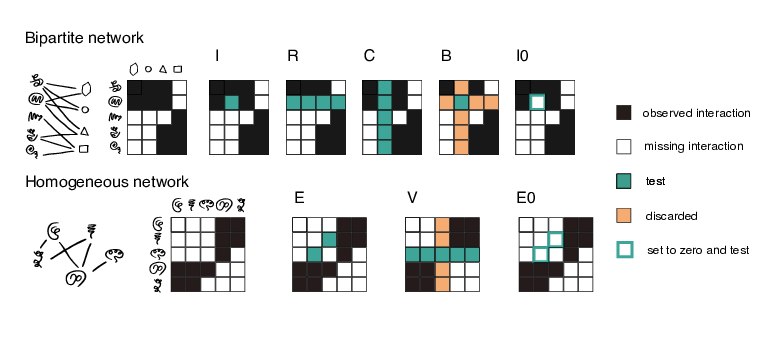
\includegraphics{Fig_settings.png}
\caption{Illustration of the different leave-one-out cross-validation
settings provided in \texttt{xnet} Figure lifted from
\citet{Stock2018cvshortcuts}. .\label{fig:CV}}
\end{figure}

In addition to the cross-validation schemes, \texttt{xnet} also provides
permutation-based methods to analyze the models. Here, the Gram matrices
\(K\), \(G\) or both are randomly permutated, i.e., the row and
corresponding columns of the Gram matrices are re-arranged in an
arbitrary order. This destroys the link between the objects and their
kernel-function. The decrease in model performance in leave-one-out
cross-validation can be recorded. The average decrease in performance
over several repetitions is an indication for which kernel is most
relevant for which prediction setting.

\hypertarget{use-of-the-package}{%
\section{Use of the package}\label{use-of-the-package}}

\label{sec:useofpackage}

For the illustrations, we use two different datasets.

The dataset \texttt{drugtarget}, first presented by
\citet{Yamanishi2008}, serves as an example of a bipartite network. It
is a small dataset containing all binary interactions between 26 nuclear
receptor protein targets and 54 drug-like compounds. To get a suitable
kernel matrix, we recomputed the kernel matrices as explained in the
vignette
\texttt{{[}Preparation\ of\ the\ example\ data{]}(../doc/Preparation\_example\_data.html)}.

The processed dataset consists of three matrices:

\begin{itemize}
\tightlist
\item
  the adjacency matrix \texttt{drugTargetInteraction};
\item
  the kernel matrix for the targets \texttt{targetSim};
\item
  the kernel matrix for the drugs \texttt{drugSim}.
\end{itemize}

The example dataset \texttt{proteinInteraction} originates from a
publication by \citet{Yamanishi2004}. It contains data on the
interactions between a subset of 769 proteins, and consists of two
objects:

\begin{itemize}
\tightlist
\item
  the adjacency matrix \texttt{proteinInteraction} where 1 indicates an
  interaction between proteins;
\item
  the kernel matrix \texttt{Kmat\_y2h\_sc} describing the similarity
  between the proteins, based on the two-hybrid method.
\end{itemize}

\hypertarget{fitting-a-two-step-kernel-ridge-regression}{%
\subsection{Fitting a two-step kernel ridge
regression}\label{fitting-a-two-step-kernel-ridge-regression}}

\hypertarget{bipartite-networks}{%
\subsubsection{Bipartite networks}\label{bipartite-networks}}

One can fit a two-step kernel ridge regression using the function
\texttt{tskrr()}. This function requires the tuning parameters
\texttt{lambda}, as explained earlier. The user can choose to set one
lambda for tuning \(K\) and \(G\) using the same lambda value, or she
can specify a different lambda for \(K\) and \(G\).

\begin{CodeChunk}

\begin{CodeInput}
R> library(xnet)
\end{CodeInput}

\begin{CodeOutput}

Attaching package: 'xnet'
\end{CodeOutput}

\begin{CodeOutput}
The following object is masked from 'package:stats':

    hat
\end{CodeOutput}
\end{CodeChunk}

\begin{CodeChunk}

\begin{CodeInput}
R> data(drugtarget)
R> 
R> drugmodel <- tskrr(y = drugTargetInteraction,
R+                    k = targetSim,
R+                    g = drugSim,
R+                    lambda = c(0.01,0.1))
R> 
R> drugmodel
\end{CodeInput}

\begin{CodeOutput}
Heterogenous two-step kernel ridge regression
---------------------------------------------
Dimensions: 26 x 54 
Lambda:
   k    g 
0.01 0.10 

Row Labels:"hsa190" "hsa2099" "hsa2100" "hsa2101" "hsa2103" ...
Col Labels:"D00040" "D00066" "D00067" "D00075" "D00088" "D00094" ...
\end{CodeOutput}
\end{CodeChunk}

\hypertarget{homogenous-network}{%
\subsubsection{Homogenous network}\label{homogenous-network}}

For homogenous networks, the same function as for bipartite networks can
be used. When no matrix \(G\) is provided, and the matrix \(Y\) is
square, TSKRR for homogeneous networks will be fitted automatically. In
this case, a single regularization parameter is provided:

\begin{CodeChunk}

\begin{CodeInput}
R> data(proteinInteraction)
R> 
R> proteinmodel <- tskrr(proteinInteraction,
R+                       k = Kmat_y2h_sc,
R+                       lambda = 0.01)
R> 
R> proteinmodel
\end{CodeInput}

\begin{CodeOutput}
Homogenous two-step kernel ridge regression
-------------------------------------------
Dimensions: 150 x 150 
Lambda:
   k 
0.01 

Labels:"YER171W" "YEL002C" "YJL210W" "YBR097W" "YHR174W" ...
\end{CodeOutput}
\end{CodeChunk}

\hypertarget{extracting-information-from-a-model.}{%
\subsubsection{Extracting information from a
model.}\label{extracting-information-from-a-model.}}

The relevant information of a TSKRR model can be extracted using various
specific functions:

\begin{itemize}
\tightlist
\item
  \texttt{lambda} returns a vector with the lambda values used;
\item
  \texttt{dim} returns the dimensions;
\item
  \texttt{labels} returns a list with two elements, \texttt{k} and
  \texttt{g}, containing the labels for the rows resp. the columns;
\item
  the functions \texttt{rownames()} and \texttt{colnames()} extract the
  labels.
\end{itemize}

\begin{CodeChunk}

\begin{CodeInput}
R> lambda(drugmodel)  # extract lambda values
\end{CodeInput}

\begin{CodeOutput}
   k    g 
0.01 0.10 
\end{CodeOutput}

\begin{CodeInput}
R> lambda(proteinmodel)
\end{CodeInput}

\begin{CodeOutput}
   k 
0.01 
\end{CodeOutput}

\begin{CodeInput}
R> dim(drugmodel) # extract the dimensions
\end{CodeInput}

\begin{CodeOutput}
[1] 26 54
\end{CodeOutput}

\begin{CodeInput}
R> protlabels <- labels(proteinmodel)
R> str(protlabels)
\end{CodeInput}

\begin{CodeOutput}
List of 2
 $ k: chr [1:150] "YER171W" "YEL002C" "YJL210W" "YBR097W" ...
 $ g: chr [1:150] "YER171W" "YEL002C" "YJL210W" "YBR097W" ...
\end{CodeOutput}
\end{CodeChunk}

The functions \texttt{fitted()} and \texttt{predict()} can be used to
extract the fitted values. The latter also allows specifying new kernel
matrices to predict for new objects in the network. To get the
residuals, one can use the function \texttt{residuals()}.

\hypertarget{performing-leave-one-out-cross-validation}{%
\subsection{Performing leave-one-out
cross-validation}\label{performing-leave-one-out-cross-validation}}

\hypertarget{settings-for-loo}{%
\subsubsection{Settings for LOO}\label{settings-for-loo}}

The most significant contribution of this package, are the various
shortcuts for leave-one-out cross-validation (LOO-CV) described by
\citet{Stock2018cvshortcuts}. Generally, LOO-CV removes a value, refits
the model, and predicts the removed value based on this refit model. In
this package, you do this using the function \texttt{loo()}. A user can
specify the cross-validation scheme using the argument
\texttt{exclusion}:

\begin{itemize}
\tightlist
\item
  \emph{interaction}: in this setting, only the interaction between two
  nodes is removed from the adjacency matrix.
\item
  \emph{row}: in this setting, the entire row for that node is removed
  from the adjacency matrix. This boils down to removing a node from the
  set \(\mathcal{U}\).
\item
  \emph{column}: in this setting, the entire column for that node is
  removed from the adjacency matrix. This boils down to removing a node
  from the set \(\mathcal{V}\).
\item
  \emph{both}: in this setting, both rows and columns are removed, i.e.,
  for every loo value the respective nodes are removed from both the
  \(\mathcal{U}\) and the \(\mathcal{V}\) set.
\end{itemize}

In the case of observational data, not observing an interaction (a zero
in the adjacency matrix) is no proof of the absence of the interaction
in practice. In those cases, it is more sensible to compute the LOO
values by replacing the interaction by 0 instead of removing it. This is
done by setting \texttt{replaceby0\ =\ TRUE} and it will use the I0 and
E0 cross-validation schemes for bipartite and homogeneous networks,
respectively.

\begin{CodeChunk}

\begin{CodeInput}
R> loo_drugs_interaction <- loo(drugmodel, exclusion = "interaction",
R+                        replaceby0 = TRUE)
R> loo_protein_both <- loo(proteinmodel, exclusion = "both")
\end{CodeInput}
\end{CodeChunk}

In both cases, the result is a matrix with the LOO values.

\hypertarget{use-loo-in-other-functions}{%
\subsubsection{Use LOO in other
functions}\label{use-loo-in-other-functions}}

Several functions use the predictions obtained by cross-validation. For
example, the residuals based on LOO values can be directly computed
using the function \texttt{residuals()}:

\begin{CodeChunk}

\begin{CodeInput}
R> loo_resid <- residuals(drugmodel, method = "loo",
R+                        exclusion = "interaction",
R+                        replaceby0 = TRUE)
R> all.equal(loo_resid,
R+           response(drugmodel) - loo_drugs_interaction )
\end{CodeInput}

\begin{CodeOutput}
[1] TRUE
\end{CodeOutput}
\end{CodeChunk}

Every other function that can use LOO values instead of predictions will
have the same two arguments \texttt{exclusion} and \texttt{replaceby0}.

\hypertarget{a-look-at-the-model-output}{%
\subsection{A look at the model
output}\label{a-look-at-the-model-output}}

The function provides a \texttt{plot()} function for looking at the
model output. This function can show you the fitted values, the LOO
values, or the residuals. It also lets you construct dendrograms based
on the \(K\) and \(G\) matrices, so you have both the predictions and
the similarity information on the nodes in one plot.

\begin{CodeChunk}

\begin{CodeInput}
R> plot(drugmodel, main = "Drug Target interaction")
\end{CodeInput}


\begin{center}\includegraphics{xnet_JSSPaper_files/figure-latex/plot-model-1} \end{center}

\end{CodeChunk}

To plot LOO values, the user set the argument \texttt{which}. As fitting
the protein model is pretty expensive, one can remove the dendrogram and
select a number of objects for closer inspection.

\begin{CodeChunk}

\begin{CodeInput}
R> plot(proteinmodel, dendro = "none", main = "Protein interaction - LOO",
R+      which = "loo", exclusion = "both",
R+      rows = rownames(proteinmodel)[10:20],
R+      cols = colnames(proteinmodel)[30:35])
\end{CodeInput}


\begin{center}\includegraphics{xnet_JSSPaper_files/figure-latex/plot-loo-values-1} \end{center}

\end{CodeChunk}

Both the breaks used for the color code and the color code itself can
also be specified.

\hypertarget{tuning-a-model-to-find-the-best-hyperparameters}{%
\subsection{Tuning a model to find the best
hyperparameters}\label{tuning-a-model-to-find-the-best-hyperparameters}}

\hypertarget{bipartite-networks-1}{%
\subsubsection{Bipartite networks}\label{bipartite-networks-1}}

In most cases, the user does not know how to the regularization
hyperparameter values for \(\lambda_u\) and \(\lambda_v\) for optimal
predictions. To find the best \texttt{lambda} values, the function
\texttt{tune()} allows one to perform a grid search. This grid search
can be specified in several ways:

\begin{itemize}
\tightlist
\item
  by specifying actual values to be tested;
\item
  by specifying the minimum and maximum lambda together with the number
  of values needed in every dimension. The function will create a grid
  that is evenly spaced on a logarithmic scale.
\end{itemize}

Tuning minimizes a loss function. Two standard loss functions are
provided, i.e., one based on mean squared error (\texttt{loss\_mse}) and
one based on the area under the ROC curve (\texttt{loss\_auc}). Any
arbitrary loss function can be specified, as long as lower values
correspond to a better model.

For heterogeneous networks, the tuning works as follows. The function
\texttt{tune()} performs a two-dimensional grid search. To do a
one-dimensional grid search (i.e., use the same value for \(\lambda_u\)
and \(\lambda_v\)), you set the argument \texttt{onedim\ =\ TRUE}. We
found that this led to only a slight decrease in performance in
practice.

\begin{CodeChunk}

\begin{CodeInput}
R> drugtuned1d <- tune(drugmodel,
R+                     lim = c(0.001,10),
R+                     ngrid = 20,
R+                     fun = loss_auc,
R+                     onedim = TRUE)
R> plot_grid(drugtuned1d, main = "1D search")
\end{CodeInput}


\begin{center}\includegraphics{xnet_JSSPaper_files/figure-latex/unnamed-chunk-1-1} \end{center}

\end{CodeChunk}

When performing a two-dimensional grid search, you can specify different
limits and grid values or lambda values for both dimensions. You do this
by passing a list with two elements for the respective arguments.

\begin{CodeChunk}

\begin{CodeInput}
R> drugtuned2d <- tune(drugmodel,
R+                      lim = list(k = c(0.001,10), g = c(0.0001,10)),
R+                      ngrid = list(k = 20, g = 10),
R+                      fun = loss_auc)
\end{CodeInput}
\end{CodeChunk}

the \texttt{plot\_grid()} function will give you a heatmap indicating
where the optimal lambda values are found:

\begin{CodeChunk}

\begin{CodeInput}
R> plot_grid(drugtuned2d, main = "2D search")
\end{CodeInput}


\begin{center}\includegraphics{xnet_JSSPaper_files/figure-latex/plot-grid-2d-model-1} \end{center}

\end{CodeChunk}

The function \texttt{lambda()} returns the best lambda values found by
the grid search.

\begin{CodeChunk}

\begin{CodeInput}
R> lambda(drugtuned1d)
\end{CodeInput}

\begin{CodeOutput}
        k         g 
0.3359818 0.3359818 
\end{CodeOutput}

\begin{CodeInput}
R> lambda(drugtuned2d)
\end{CodeInput}

\begin{CodeOutput}
        k         g 
0.2069138 0.2154435 
\end{CodeOutput}
\end{CodeChunk}

In this case, a one-dimensional grid search gives relatively different
optimal lambda values. To get more information on the loss values, one
can use the function \texttt{get\_loss\_values()}. This allows one to
examine the actual improvement for every lambda value. The output is
always a matrix, and in the case of a 1D search, it is a matrix with one
column. Combining these values with the lambda grid shows that the
difference between a lambda value of around 0.20 and around 0.34 is
minimal. This is also obvious from the grid plots shown above.

\begin{CodeChunk}

\begin{CodeInput}
R> cbind(
R+   loss = get_loss_values(drugtuned1d)[,1],
R+   lambda = get_grid(drugtuned1d)$k
R+ )[10:15,]
\end{CodeInput}

\begin{CodeOutput}
          loss    lambda
[1,] 0.1275495 0.0784760
[2,] 0.1239134 0.1274275
[3,] 0.1219094 0.2069138
[4,] 0.1217656 0.3359818
[5,] 0.1238880 0.5455595
[6,] 0.1271689 0.8858668
\end{CodeOutput}
\end{CodeChunk}

\hypertarget{homogenous-networks}{%
\subsubsection{Homogenous networks}\label{homogenous-networks}}

Homogenous networks have a single lambda value, and should hence only
search in a single dimension. The following code tests 20 lambda values
between 0.001 and 10.

\begin{CodeChunk}

\begin{CodeInput}
R> proteintuned <- tune(proteinmodel,
R+                      lim = c(0.0001,10),
R+                      ngrid = 20,
R+                      fun = loss_auc)
R> proteintuned
\end{CodeInput}

\begin{CodeOutput}
Tuned homogenous two-step kernel ridge regression
-------------------------------------------------
Dimensions: 150 x 150 
Lambda:
           k 
0.0001832981 

Labels:"YER171W" "YEL002C" "YJL210W" "YBR097W" "YHR174W" ...

Tuning information:
-------------------
exclusion setting: interaction 
loss value: 0.3315376 
loss function: Area under curve (loss_auc) 
\end{CodeOutput}
\end{CodeChunk}

The returned object is again a model object with the model fitted using
the best lambda value. It also contains extra information on the
settings of the tuning. The user can extract the grid values as follows:

\begin{CodeChunk}

\begin{CodeInput}
R> get_grid(proteintuned)
\end{CodeInput}

\begin{CodeOutput}
$k
 [1] 1.000000e-04 1.832981e-04 3.359818e-04 6.158482e-04 1.128838e-03
 [6] 2.069138e-03 3.792690e-03 6.951928e-03 1.274275e-02 2.335721e-02
[11] 4.281332e-02 7.847600e-02 1.438450e-01 2.636651e-01 4.832930e-01
[16] 8.858668e-01 1.623777e+00 2.976351e+00 5.455595e+00 1.000000e+01
\end{CodeOutput}
\end{CodeChunk}

This returns a list with one or two elements, each element containing
the grid values for the respective kernel matrix.

It is easy to create a plot to inspect the tuning visually:

\begin{CodeChunk}

\begin{CodeInput}
R> plot_grid(proteintuned)
\end{CodeInput}


\begin{center}\includegraphics{xnet_JSSPaper_files/figure-latex/plot-grid-1} \end{center}

\end{CodeChunk}

This object is also a \texttt{tskrr} model, so all the functions used
above can be used here as well. For example, we can use the same code as
before to inspect the LOO values of this tuned model:

\begin{CodeChunk}

\begin{CodeInput}
R> plot(proteintuned, dendro = "none", main = "Protein interaction - LOO",
R+      which = "loo", exclusion = "both",
R+      rows = rownames(proteinmodel)[10:20],
R+      cols = colnames(proteinmodel)[30:35])
\end{CodeInput}


\begin{center}\includegraphics{xnet_JSSPaper_files/figure-latex/residuals-tuned-model-1} \end{center}

\end{CodeChunk}

\hypertarget{making-predictions}{%
\subsection{Making predictions}\label{making-predictions}}

The main reason for building a pairwise model is to make predictions for
new objects. To make predictions using a \texttt{tskrr} model, the
values of the two kernel functions between the objects in the training
data and the new objects need to be computed.

\begin{CodeChunk}

\begin{CodeInput}
R> idk_test <- c(5,10,15,20,25)
R> idg_test <- c(2,4,6,8,10)
R> 
R> drugInteraction_train <- drugTargetInteraction[-idk_test, -idg_test]
R> target_train <- targetSim[-idk_test, -idk_test]
R> drug_train <- drugSim[-idg_test, -idg_test]
R> 
R> target_test <- targetSim[idk_test, -idk_test]
R> drug_test <- drugSim[idg_test, -idg_test]
\end{CodeInput}
\end{CodeChunk}

The following drugs and targets are removed from the training data and
will be used for predictions later:

\begin{CodeChunk}

\begin{CodeInput}
R> rownames(target_test)
\end{CodeInput}

\begin{CodeOutput}
[1] "hsa2103" "hsa4306" "hsa5915" "hsa6256" "hsa9970"
\end{CodeOutput}

\begin{CodeInput}
R> colnames(drug_test)
\end{CodeInput}

\begin{CodeOutput}
 [1] "D00040" "D00067" "D00088" "D00105" "D00143" "D00182" "D00187"
 [8] "D00188" "D00211" "D00246" "D00279" "D00299" "D00312" "D00316"
[15] "D00327" "D00348" "D00443" "D00462" "D00506" "D00554" "D00565"
[22] "D00577" "D00585" "D00586" "D00596" "D00627" "D00690" "D00730"
[29] "D00898" "D00930" "D00950" "D00951" "D00954" "D00956" "D00961"
[36] "D00962" "D00965" "D01115" "D01132" "D01161" "D01217" "D01294"
[43] "D01387" "D01441" "D01689" "D02217" "D02367" "D04066" "D05341"
\end{CodeOutput}
\end{CodeChunk}

We can now train the data using \texttt{tune()} just like we would use
\texttt{tskrr()}

\begin{CodeChunk}

\begin{CodeInput}
R> trained <- tune(drugInteraction_train,
R+                 k = target_train,
R+                 g = drug_train,
R+                 ngrid = 30)
\end{CodeInput}
\end{CodeChunk}

\hypertarget{predicting-new-rows}{%
\subsubsection{Predicting new rows}\label{predicting-new-rows}}

To predict the interaction between new targets and the drugs in the
model, we need to pass the kernel values for the similarities between
the new targets and the ones in the model. The \texttt{predict()}
function will select the correct \textbf{G} matrix for calculating the
predictions.

\begin{CodeChunk}

\begin{CodeInput}
R> Newtargets <- predict(trained, k = target_test)
R> Newtargets[, 1:5]
\end{CodeInput}

\begin{CodeOutput}
             D00040     D00067      D00088     D00105      D00143
hsa2103 0.004057079 0.03081055 0.009556427 0.04742997 0.008212541
hsa4306 0.001703995 0.02759991 0.175792592 0.04809118 0.024805465
hsa5915 0.023949572 0.01421044 0.008865099 0.01646451 0.016024808
hsa6256 0.010536788 0.02970235 0.018628412 0.03806541 0.003662778
hsa9970 0.015759320 0.02500044 0.035086840 0.04464471 0.181819822
\end{CodeOutput}
\end{CodeChunk}

\hypertarget{predicting-new-columns}{%
\subsubsection{Predicting new columns}\label{predicting-new-columns}}

If one wants to predict for new rows (e.g., drugs), you need the kernel
values for the similarities between new drugs and the drugs trained in
the model.

\begin{CodeChunk}

\begin{CodeInput}
R> Newdrugs <- predict(trained, g = drug_test)
R> Newdrugs[1:5, ]
\end{CodeInput}

\begin{CodeOutput}
               D00066       D00075       D00094        D00129
hsa190   0.0004385072 3.910979e-05 0.0000317464  5.801116e-04
hsa2099  0.0268199330 3.264114e-01 0.0227098621 -1.072246e-01
hsa2100 -0.0289764612 3.207540e-01 0.0147790518 -1.264217e-01
hsa2101 -0.0048777886 1.309579e-02 0.0090779102  4.106452e-06
hsa2104 -0.0051459974 1.258277e-02 0.0095775683  1.577701e-05
               D00163
hsa190   0.0003651196
hsa2099  0.0623070092
hsa2100 -0.1383998327
hsa2101 -0.0593089366
hsa2104 -0.0596787553
\end{CodeOutput}
\end{CodeChunk}

\hypertarget{predict-for-new-rows-and-columns}{%
\subsubsection{Predict for new rows and
columns}\label{predict-for-new-rows-and-columns}}

You can combine both kernel matrices used above to get predictions about
the interaction between new drugs and new targets:

\begin{CodeChunk}

\begin{CodeInput}
R> Newdrugtarget <- predict(trained, k=target_test, g=drug_test)
R> Newdrugtarget
\end{CodeInput}

\begin{CodeOutput}
               D00066     D00075       D00094       D00129        D00163
hsa2103  7.715195e-03 0.02921056 -0.012015102  0.008404732 -4.006168e-02
hsa4306  1.134892e-01 0.13809671  0.002077053 -0.024120960  2.336087e-02
hsa5915 -1.173301e-05 0.02535359  0.423718351  0.012963952 -1.475475e-02
hsa6256  2.490618e-02 0.03032823  0.063798137  0.005722959  5.630761e-05
hsa9970  5.919073e-02 0.02541274  0.031471514  0.135712388  5.288650e-02
\end{CodeOutput}
\end{CodeChunk}

\hypertarget{impute-new-values-based-on-a-tskrr-model}{%
\subsection{Impute new values based on a tskrr
model}\label{impute-new-values-based-on-a-tskrr-model}}

Sometimes you have missing values in an adjacency matrix. These missing
values can be imputed based on the simple iterative algorithm described
earlier.

Apart from the usual arguments of \texttt{tskrr}, you can give
additional parameters to the function \texttt{impute\_tskrr}. The most
important ones are

\begin{itemize}
\tightlist
\item
  \texttt{niter}: the maximum number of iterations;
\item
  \texttt{tol}: the tolerance, i.e., the minimal sum of squared
  differences between iteration steps to keep the algorithm going;
\item
  \texttt{verbose}: setting this to 1 or 2 gives additional info on the
  algorithm performance.
\end{itemize}

We illustrate this on a dataset with missing values:

\begin{CodeChunk}

\begin{CodeInput}
R> drugTargetMissing <- drugTargetInteraction
R> idmissing <- c(10,20,30,40,50,60)
R> drugTargetMissing[idmissing] <- NA
\end{CodeInput}
\end{CodeChunk}

We can now try to impute these values. The outcome is again a tskrr
model.

\begin{CodeChunk}

\begin{CodeInput}
R> imputed <- impute_tskrr(drugTargetMissing,
R+                         k = targetSim,
R+                         g = drugSim,
R+                         verbose = TRUE)
\end{CodeInput}

\begin{CodeOutput}
Nr. of iterations: 80 - Deviation:1.4900616992948e-08
\end{CodeOutput}

\begin{CodeInput}
R> plot(imputed, dendro = "none")
\end{CodeInput}


\begin{center}\includegraphics{xnet_JSSPaper_files/figure-latex/unnamed-chunk-8-1} \end{center}

\end{CodeChunk}

To extract information on the imputation, several functions are
available:

\begin{itemize}
\tightlist
\item
  \texttt{has\_imputed\_values()} tells you whether the model contains
  imputed values;
\item
  \texttt{is\_imputed()} returns a logical matrix where \texttt{TRUE}
  indicates an imputed value;
\item
  \texttt{which\_imputed()} returns an integer vector with the positions
  of the imputed values. Note that these positions are vector positions,
  i.e., they give the position in a single dimension (according to how a
  matrix is stored internally in R).
\end{itemize}

\begin{CodeChunk}

\begin{CodeInput}
R> has_imputed_values(imputed)
\end{CodeInput}

\begin{CodeOutput}
[1] TRUE
\end{CodeOutput}

\begin{CodeInput}
R> which_imputed(imputed)
\end{CodeInput}

\begin{CodeOutput}
[1] 10 20 30 40 50 60
\end{CodeOutput}

\begin{CodeInput}
R> # Extract only the imputed values
R> id <- is_imputed(imputed)
R> predict(imputed)[id]
\end{CodeInput}

\begin{CodeOutput}
[1]  0.17454499  0.03111647 -0.01402729 -0.03812844  0.28626726  0.06590431
\end{CodeOutput}
\end{CodeChunk}

\hypertarget{related-software}{%
\section{Related software}\label{related-software}}

\label{sec:relatedsoftware}

Pairwise learning is a viable approach for various machine learning
problems, including network inference, missing value imputation,
collaborative filtering, multi-task learning, transfer learning,
zero-shot learning, etc. These problems can all be posed as a supervised
network prediction problem, or, equivalently, predicting values, rows,
and columns in a matrix. As such, the TSKRR model, as provided by our
\textbf{xnet} package provides similar functionality to numerous
packages.

The most conceptually similar package is \textbf{RLScore}
\citep{Pahikkala2016}, a Python library implementing many
least-squares-based kernel learning algorithms, including
Kronecker-kernel ridge regression and two-step kernel ridge regression.
Although the R programming language has several packages implementing
kernel methods, our package is the first to offer this pairwise learning
framework. Since \textbf{xnet} only provides the functions for training,
validating and visualization the TSKKR method, we recommend using other
packages for computing the kernel matrices. For example,
\textbf{kernlab} \citep{Karatzoglou2004} provides the most popular
kernels for vectorial data, \textbf{graphkernels}
\url{https://cran.r-project.org/web/packages/graphkernels/index.html}
provides kernel functions to compare graphs while the \textbf{SHOGUN}
toolbox \citep{Sonnenburg2010} provides, among other functionality,
string kernels.

Given R's large ecosystem of packages for analyzing biological data,
there exist many packages for network prediction. For example, for gene
regulatory network prediction, \textbf{SIRENE} \citep{Mordelet2008},
\textbf{minet} \citep{Meyer2008} and \textbf{Parmigene}
\citep{Sales2011} provide unsupervised methods for gene-gene interaction
prediction. The importance of correct validation is illustrated by
packages such as \textbf{NetBenchmark} \citep{Bellot2015a}, which
provide tools to test the robustness of different network inference
methods using simulators. \textbf{xnet} is a comprehensive package that
adds a supervised network prediction method to this pool of unsupervised
algorithms.

R also has packages for missing value imputation, of which \textbf{MICE}
(Multivariate Imputation by Chained Equations) \citep{VanBuuren2011} and
\textbf{MissForest} \citep{Stekhoven2012} are well-known examples. Our
package does not have the ambition to replace these. Most specialized
methods for problems such as missing value imputation will likely
outperform it, if only by a small margin. The goal of \textbf{xnet} is
to provide a single method that can handle various machine learning
problems, including missing value imputation, but also supervised
network prediction, multi-task learning, and zero-shot learning.

\hypertarget{conclusions}{%
\section{Conclusions}\label{conclusions}}

\textbf{Acknowledgements}

TBD

\textbf{Author contributions}

\begin{itemize}
\tightlist
\item
  MS outlined and contributed to the package, provided the first
  implementation, and wrote the manuscript.
\item
  JM developed the package and contributed to the manuscript.
\item
  BDB helped to outline the package and contributed to the manuscript.
\end{itemize}

\bibliography{refs.bib}


\end{document}

